\chapter{Introduction}
Every day, throughout our lives, we are required 
to believe certain things and not to believe other things. This applies not
only to the ``big questions'' of life, but also to trivial matters, and 
everything in between. For example, this morning I boarded the bus to 
university, sure that it would actually take me here and not to Wellington.
How did I know the bus would not take me to Wellington? Well, for starters
I have taken the same bus many times before and it has always taken me to the
university. Another clue was that the bus said ``Midtown'' on it, and a bus
to Wellington would probably have said Wellington, and would not have stopped
at a minor bus stop in suburban Auckland.
None of this evidence {\it proves} that the bus would take me to university,
but it does makes it plausible. Given all these pieces of information, I feel
quite certain that the bus will take me to the city. I feel so certain
about this that the possibility of an
unplanned trip to Wellington never even entered my mind until I decided to
write this paragraph.

Somehow, our brains are very often able to accurately predict the correct answer
to many questions (e.g. the destination of a bus), even though we don't have
all of the available information that we would need to be 100\% certain.
We do this using our experience of the world and our intuition, usually 
without much conscious attention or problem solving. However, there are areas
of study where we can't just use our intuition to make judgments like this.
For example, most of science involves such situations - people tend to be
interested in trying to answer questions that haven't yet been answered!
This is where statistics comes in: to help us in this grey area where we can't
be 100\% certain about things, but we want to do the best we can with our
incomplete information.

\section{Certainty, Uncertainty and Probability}
In the above example, I said things like ``I couldn't be 100\% certain''. The
idea of using a number to describe how certain you are is quite familiar.
For example, contestants on ``Who Wants to be a Millionaire'' often say things
like ``I'm about 80\% sure the answer is A''. There are some interesting
things to notice about this statement. Firstly, it is a subjective statement.
If someone else were in the seat trying to answer the question, they might say
the probability that A is correct is 100\%, because they know the answer!
A third person faced with the same question might say the probability is 25\%,
because they have no idea and only know that one of the four answers
must be correct.

In Bayesian statistics, the interpretation of what {\it probability} means is
that it is a description of {\it how certain you are that some statement is
true}.
If the probability is 1, you are sure that the statement is true. So sure, in
fact, that nothing could ever change your mind (we will demonstrate this later).
If the probability is 0, you
are sure that the statement is false. If the probability is 0.5, then you
are as uncertain as you would be about a fair coin flip. If the probability is
0.95, then you're quite sure the statement is true, but it wouldn't be {\it too}
surprising to you if you found out the statement was false. See
Figure~\ref{fig:probability_scale} for a graphical depiction of probabilities
as degrees of certainty or plausibility.

\begin{figure}
\begin{center}
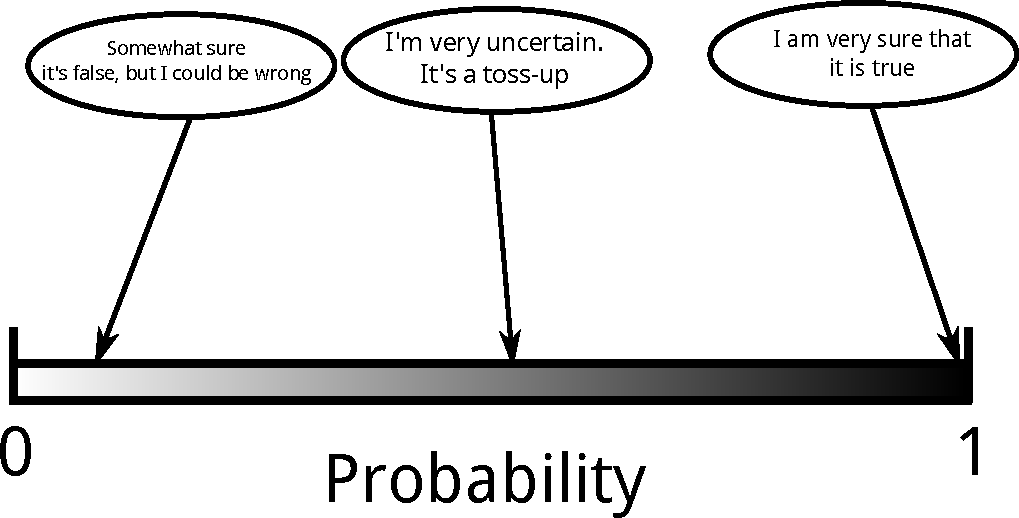
\includegraphics[scale=0.6]{Figures/probability_scale.pdf}
\caption{Probability can be used to describe degrees of certainty, or
how plausible some statement is.\label{fig:probability_scale}}
\end{center}
\end{figure}

\begin{center}
\begin{tabular}{|c|}
\hline
{\bf In Bayesian statistics, probabilities are in the mind, not in the world.}\\
\hline
\end{tabular}
\end{center}

It might sound like there is nothing more to Bayesian statistics than just
thinking about a question and then blurting out a probability that feels
appropriate. Fortunately for us, there's more to it than that! To see why, think
about how you change your mind when new evidence (such as a data set) becomes
available. For example, you may be on ``Who Wants to be a Millionaire?'' and
not know the answer to a question, so you might think the probability that it is
$A$ is 25\%. But if you call your friend using ``phone a friend'', and
your friend says
``it's definitely $A$'', then you would be more confident that it is $A$!

\begin{center}
\begin{tabular}{|c|}
\hline
{\bf When we get new information, we should {\it update} our probabilities.}\\
{\bf Bayesian methods tell us exactly how to do that.}\\
\hline
\end{tabular}
\end{center}

In this course, we will learn how to do {\it data analysis} from a Bayesian
point of view. So while the discussion in this chapter might sound a bit
like philosophy, we will see that using this kind of thinking can give us
new ways of solving practical data analysis problems. The methods we will use
will all have a common structure, so if you are faced with a completely new
data analysis problem one day, you will be able to design your own analysis
methods by using the Bayesian framework. Best of all, the methods make sense
and perform extremely well in practice!




